
%%%%%%%%%%%%%%%%%%%%%%%%%%%%%%%%%%%%%%%%%%%%%%%%%%%%%%%%%%%%%%%%%%%%%%%%%%%%%%%%%%%
\subsection{Hyperbel}\index{Hyperbel (negative Exponenten)}

(«Hyperbel» Griechisch = «über das Ziel hinaus werfen»)


Zur Erinnerung:
\begin{multicols}{2}
\begin{itemize}
	\item $x^{-1} = \frac{1}{x}$
	\item $x^{-2} = \frac{1}{x^2}$
	\item $x^{-3} = \frac{1}{x^3}$
	\item $x^{-4} = \frac{1}{x^4}$
	\item $x^{-5} = \frac{1}{x^5}$
  \item ...
\end{itemize}
\end{multicols}

Zeichnen Sie die Funktion $f: y = x^{-1}$ im Definitinosbereich
$\mathbb{D} = [-5;5]\TRAINER{\backslash \{0\}}\noTRAINER{......}$

\bbwGraph{-6}{6}{-3}{3}{%%
  \TRAINER{\bbwFunc{1/\x}{-5:-0.3}}
  \TRAINER{\bbwFunc{1/\x}{0.3:5}}

}%%

\newpage


Zeichnen Sie zusätzlich Funktion $f: y = x^{-2}$  und $x^{-3}$im Bereich $[-5;5]$:

\bbwGraph{-6}{6}{-5}{5}{%%
  % x^-2
  \TRAINER{\bbwFuncC{1/(\x * \x)}{-5:-0.447}{green}}%% 0.447 = 1/sqrt (5)
  \TRAINER{\bbwFuncC{1/(\x * \x)}{0.447:5}{green}}
  \TRAINER{\bbwLetter{2.5,0.5}{x^{-2}}{green}}
  \TRAINER{\bbwLetter{-1.5,1}{x^{-2}}{green}}

  %x^-3
  \TRAINER{\bbwFuncC{1/(\x * \x * \x)}{-5:-0.584}{blue}}
  \TRAINER{\bbwFuncC{1/(\x * \x * \x)}{0.584:5}{blue}}
  \TRAINER{\bbwLetter{0.8,0.3}{x^{-3}}{blue}}
  \TRAINER{\bbwLetter{-1.2,-3.8}{x^{-3}}{blue}}
  \TRAINER{\bbwLetter{1.2,4.5}{x^{-3}}{blue}}

}%%

\begin{definition}{Hyperbel}{definition_hyperbel}
  Der Graph einer Potenzfunktion $$f: y=ax^z$$
  mit $z \in \{-1, -2, -3, -4, ...\}$ heißt
\textbf{Hyperbel}\index{Hyperbel} der Ordnung $z$.
\end{definition}

Der Definitionsbereich von Hyperbeln entspricht dem Definitionsbereich
des Funktionsterms. Merke: Es darf nicht durch Null geteilt werden:

$$x^{-5} = \frac{1}{x^5} \Longrightarrow \mathbb{D} = \mathbb{R} \backslash \{0\}$$


\subsection*{Aufgaben}
\GESOAadB{306ff}{19. Zeichnung mit geogebra.org, 20.
  Zeichnung mit geogebra.org, 25. b) c), 26. a) b), 27. b) c), 33*}
\TALSAadB{205}{771. a) c) d) e) g) h) j)}


\newpage

\subsubsection{Charakteristiken}
\textbf{Spiegelungen:}\\

Welche Funktionen $x$, $x^{-1}$, $x^{-2}$, $x^{-3}$ sind an welchen Achsen bzw. Punkten gespiegelt?

\renewcommand{\mmPapier}[1]{\mmPapierZwei{#1}{16.0}}
\begin{tabular}{c|p{10cm}}
  $x^{-1}$ &  \TNT{0.8}{Am Ursprung $O(0|0)$ : Punktspiegelung}\\
  \hline
  $x^{-2}$ &  \TNT{0.8}{An der $y$-Achse: Achsensymmetrie}\\
  \hline
  $x^{-3}$ &  \TNT{0.8}{Am Ursprung $O(0|0)$: Punktspiegelung}\\
  \hline
  $x^{-4}$ &  \TNT{0.8}{An der $y$-Achse: Achsensymmetrie}\\
  \hline  
\end{tabular}
\renewcommand{\mmPapier}[1]{\mmPapierZwei{#1}{17.6}}


\paragraph{Definitions- und Wertebereiche:}

Geben Sie für die obigen Funktionen an, was ihr Definitions- bzw. Wertebereich ist\footnote{Grundmenge ist $\mathbb{R}$.}:

\begin{tabular}{c|c|c}
Funktionsterm & Definitionsbereich $\mathbb{D}$& Wertebereich $\mathbb{W}$\\ \hline
  $x^{-1}$ & \TRAINER{$\mathbb{R}\backslash\{0\}$} &  \TRAINER{$\mathbb{R}\backslash\{0\}$}\\ \hline
  $x^{-2}$ & \TRAINER{$\mathbb{R}\backslash\{0\}$} &  \TRAINER{$\mathbb{R}^{+}\backslash\{0\}$}\\ \hline
  $x^{-3}$ & \TRAINER{$\mathbb{R}\backslash\{0\}$} &  \TRAINER{$\mathbb{R}\backslash\{0\}$}\\ \hline
  $x^{-4}$ & \TRAINER{$\mathbb{R}\backslash\{0\}$} &  \TRAINER{$\mathbb{R}^{+}\backslash\{0\}$}\\ \hline
\end{tabular}


\subsection*{Aufgaben}
\GESO{\aufgabenFarbe{Weitere Aufgaben im \textit{Kompendium} Kap. 3.3 S. 26. Aufg. 28-31}}
\GESO{\aufgabenFarbe{Aufgabe der Nullserie 2 (zweite Nullserie): Aufg. 7 auf Seite 3}}
\GESO{\aufgabenFarbe{Maturaprüfung 2016, Aufg. 8 (Graphen zuordnen)}}
\newpage

\subsection{Zusammenfassungen und
  Überblick}\index{Potenzfunktionen!Überblick}

$$y = a\cdot{}x^z$$

$z$ gerade: Gespiegelt an der $y$-Achse

$z$ ungerade: Gespiegelt am Ursprung $O=(0|0)$

Ist ${\color{green}a>0}$\TRAINER{ (grün in der Graphik)}, so sind Graphen mit
geraden Exponenten nach oben geöffnet bzw. mit ungeraden Exponenten im
Quadranten I und III.

Ist ${\color{red}a<0}$\TRAINER{ (rot/orange in der Graphik)}, so sind Graphen mit
geraden Exponenten nach unten geöffnet bzw. mit ungeraden Exponenten
im Quadranten II und IV.

\TNTeop{
 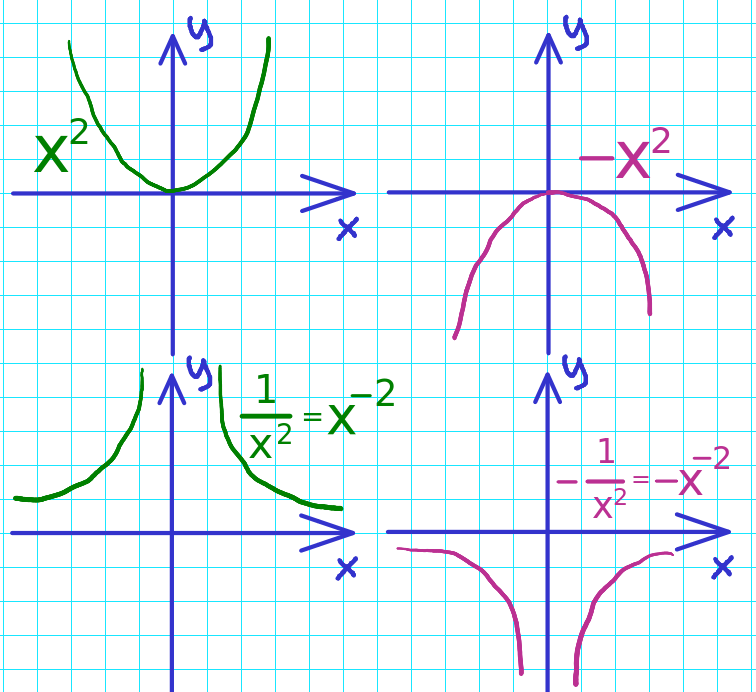
\includegraphics[width=8.5cm]{allg/funktionen/img/potenzfct/potenzFunktionenGerade.png}\hfill{}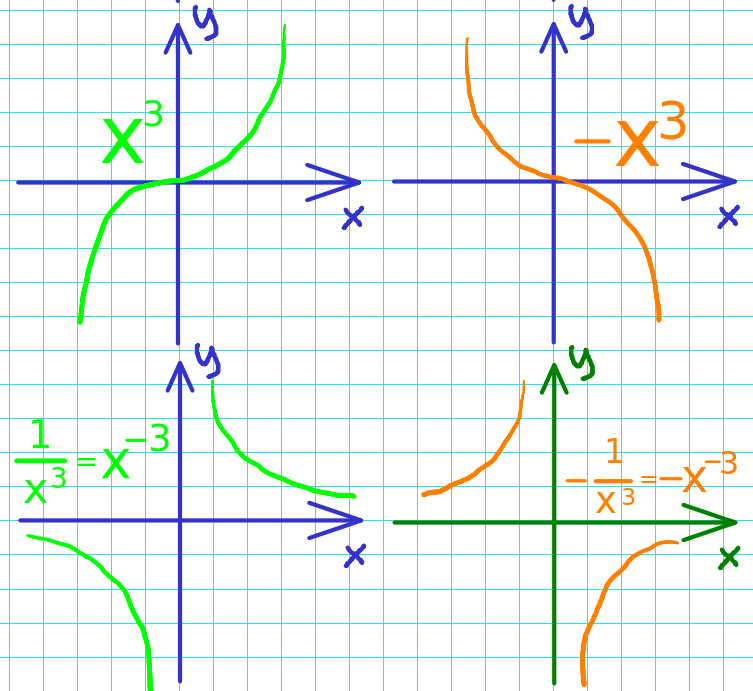
\includegraphics[width=8.5cm]{allg/funktionen/img/potenzfct/potenzFunktionenUngerade.png}
}%% END TNT

\newpage

